\documentclass[./\jobname.tex]{subfiles}
\begin{document}


\chapter{Drawings}

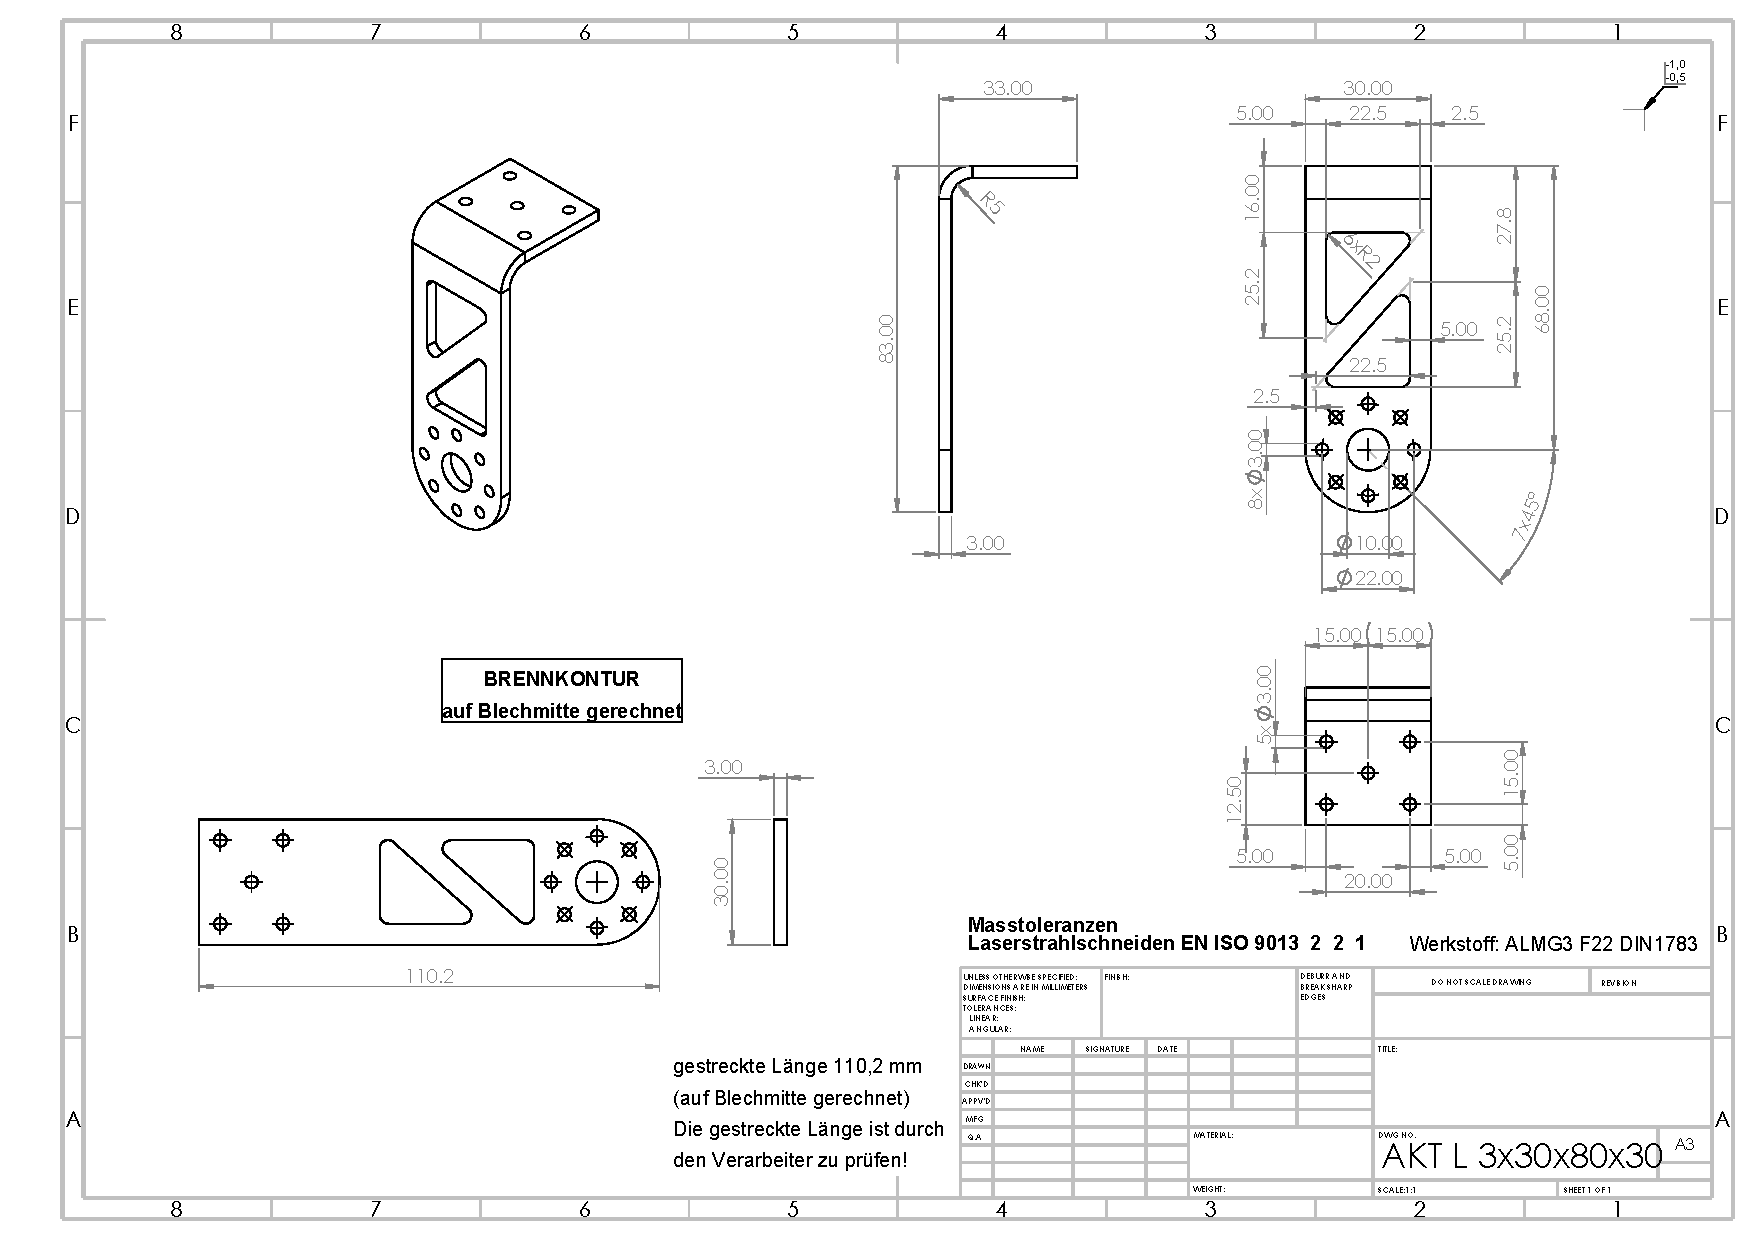
\includepdf[page=-]{../img/pdf/AKT L 3x30x80x30.pdf}
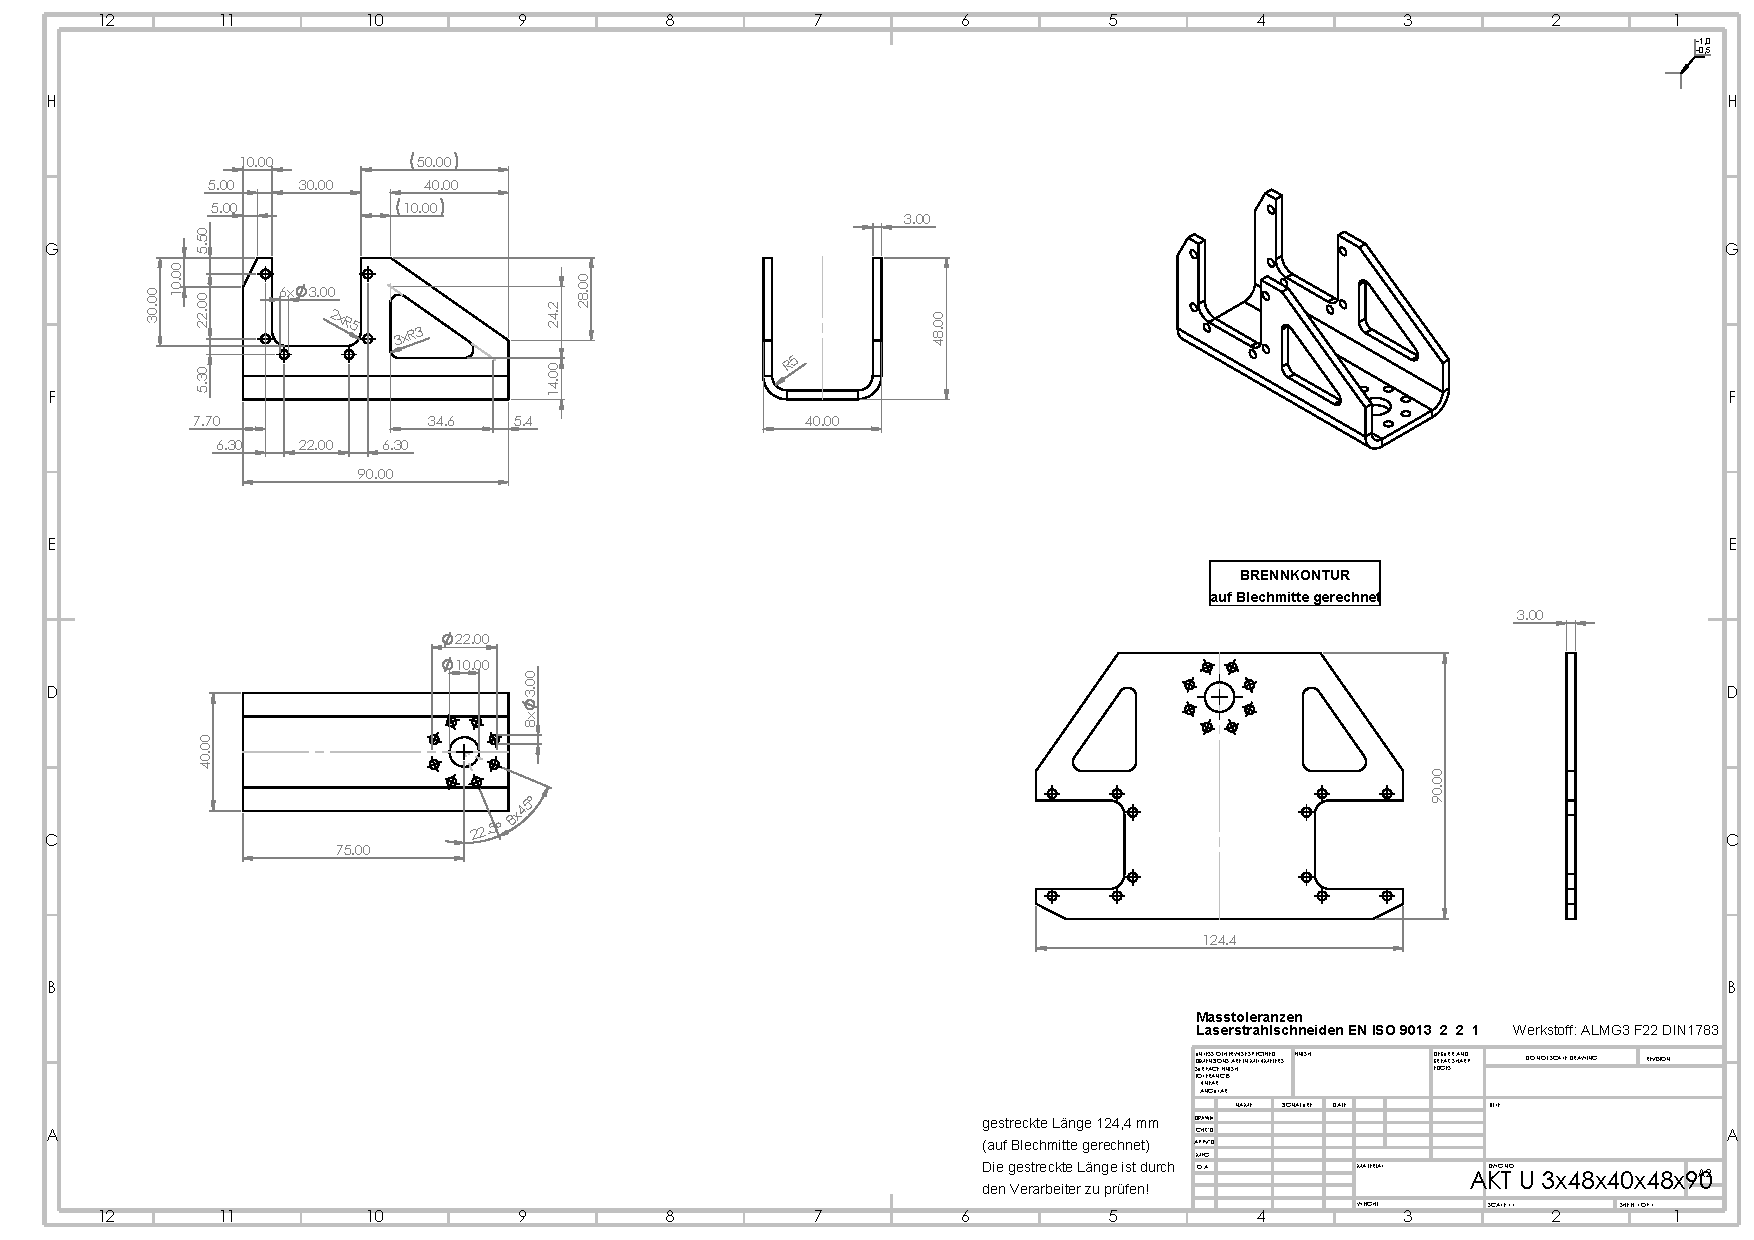
\includepdf[page=-]{../img/pdf/AKT U 3x48x40x48x90.pdf}
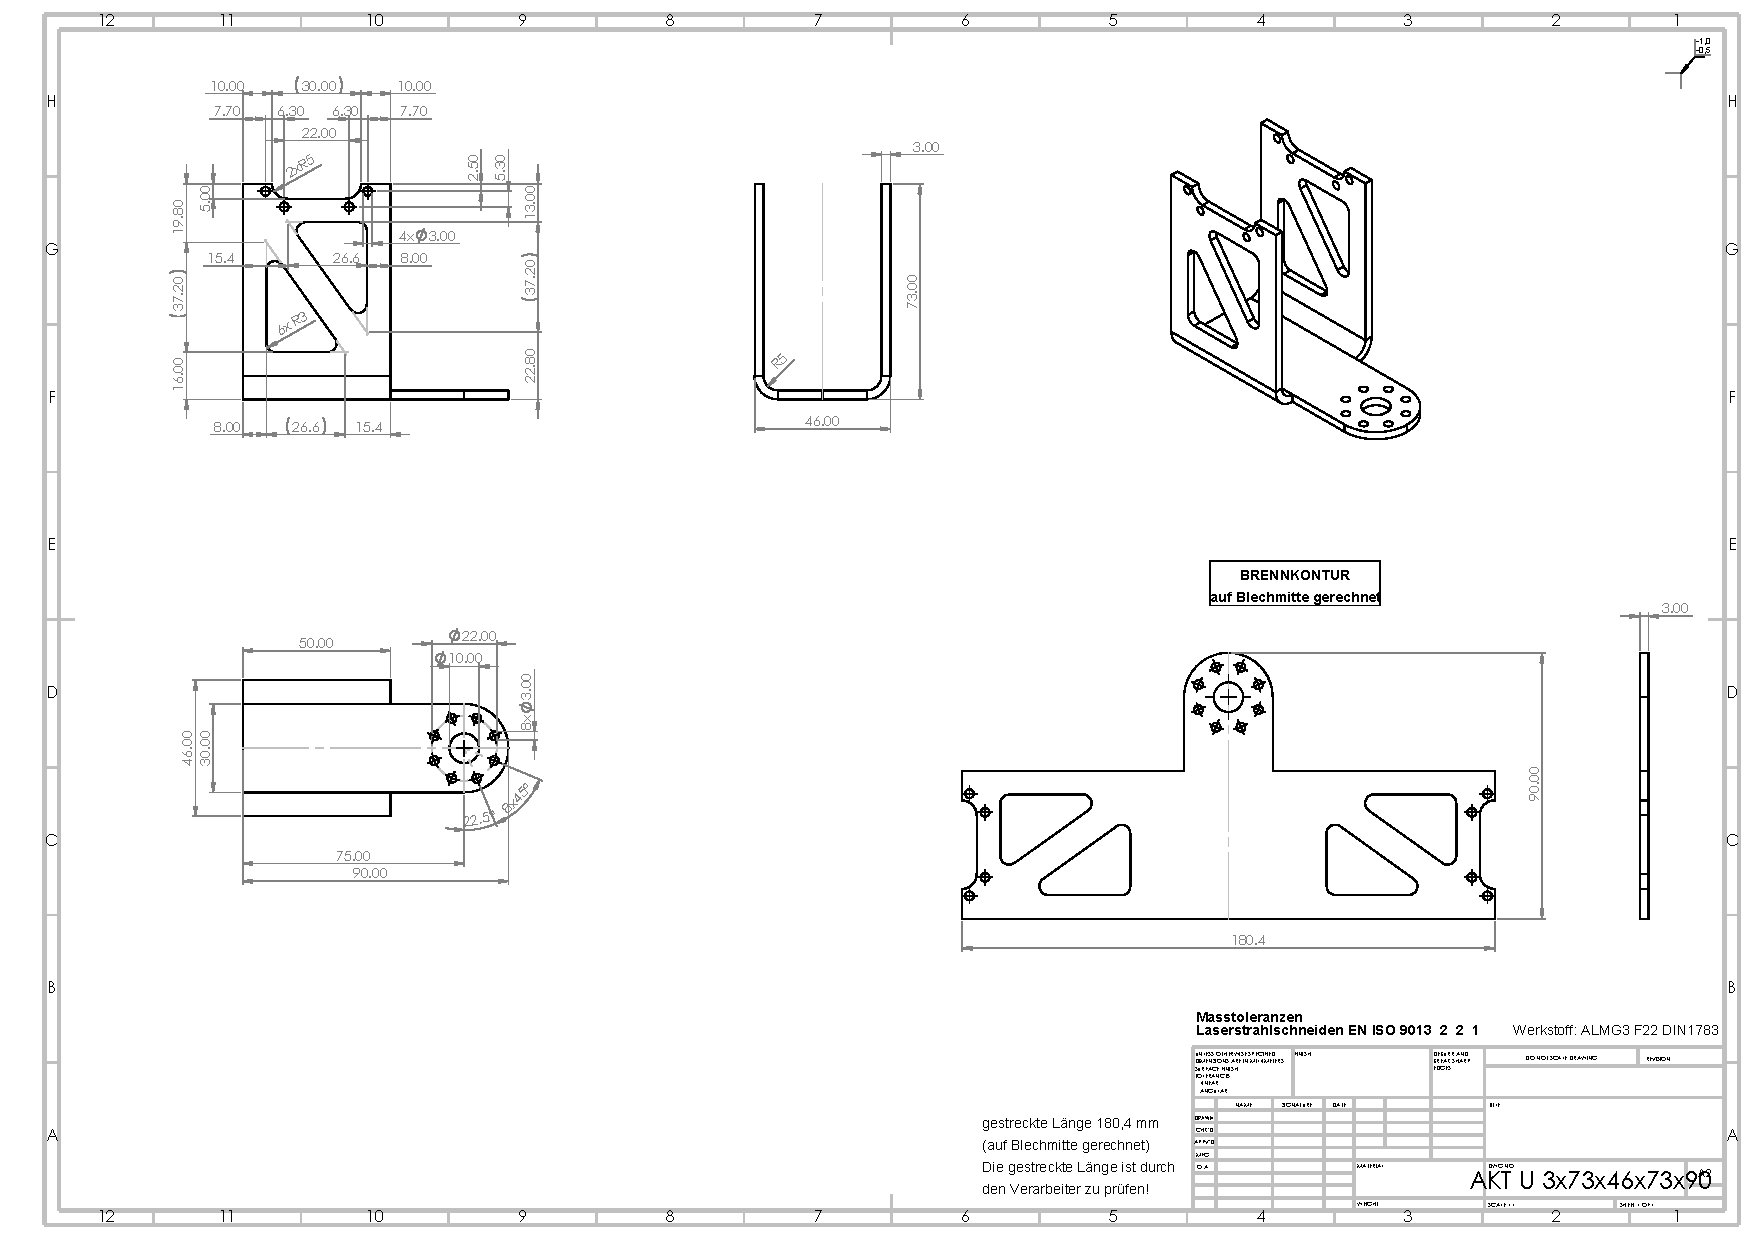
\includepdf[page=-]{../img/pdf/AKT U 3x73x46x73x90.pdf}
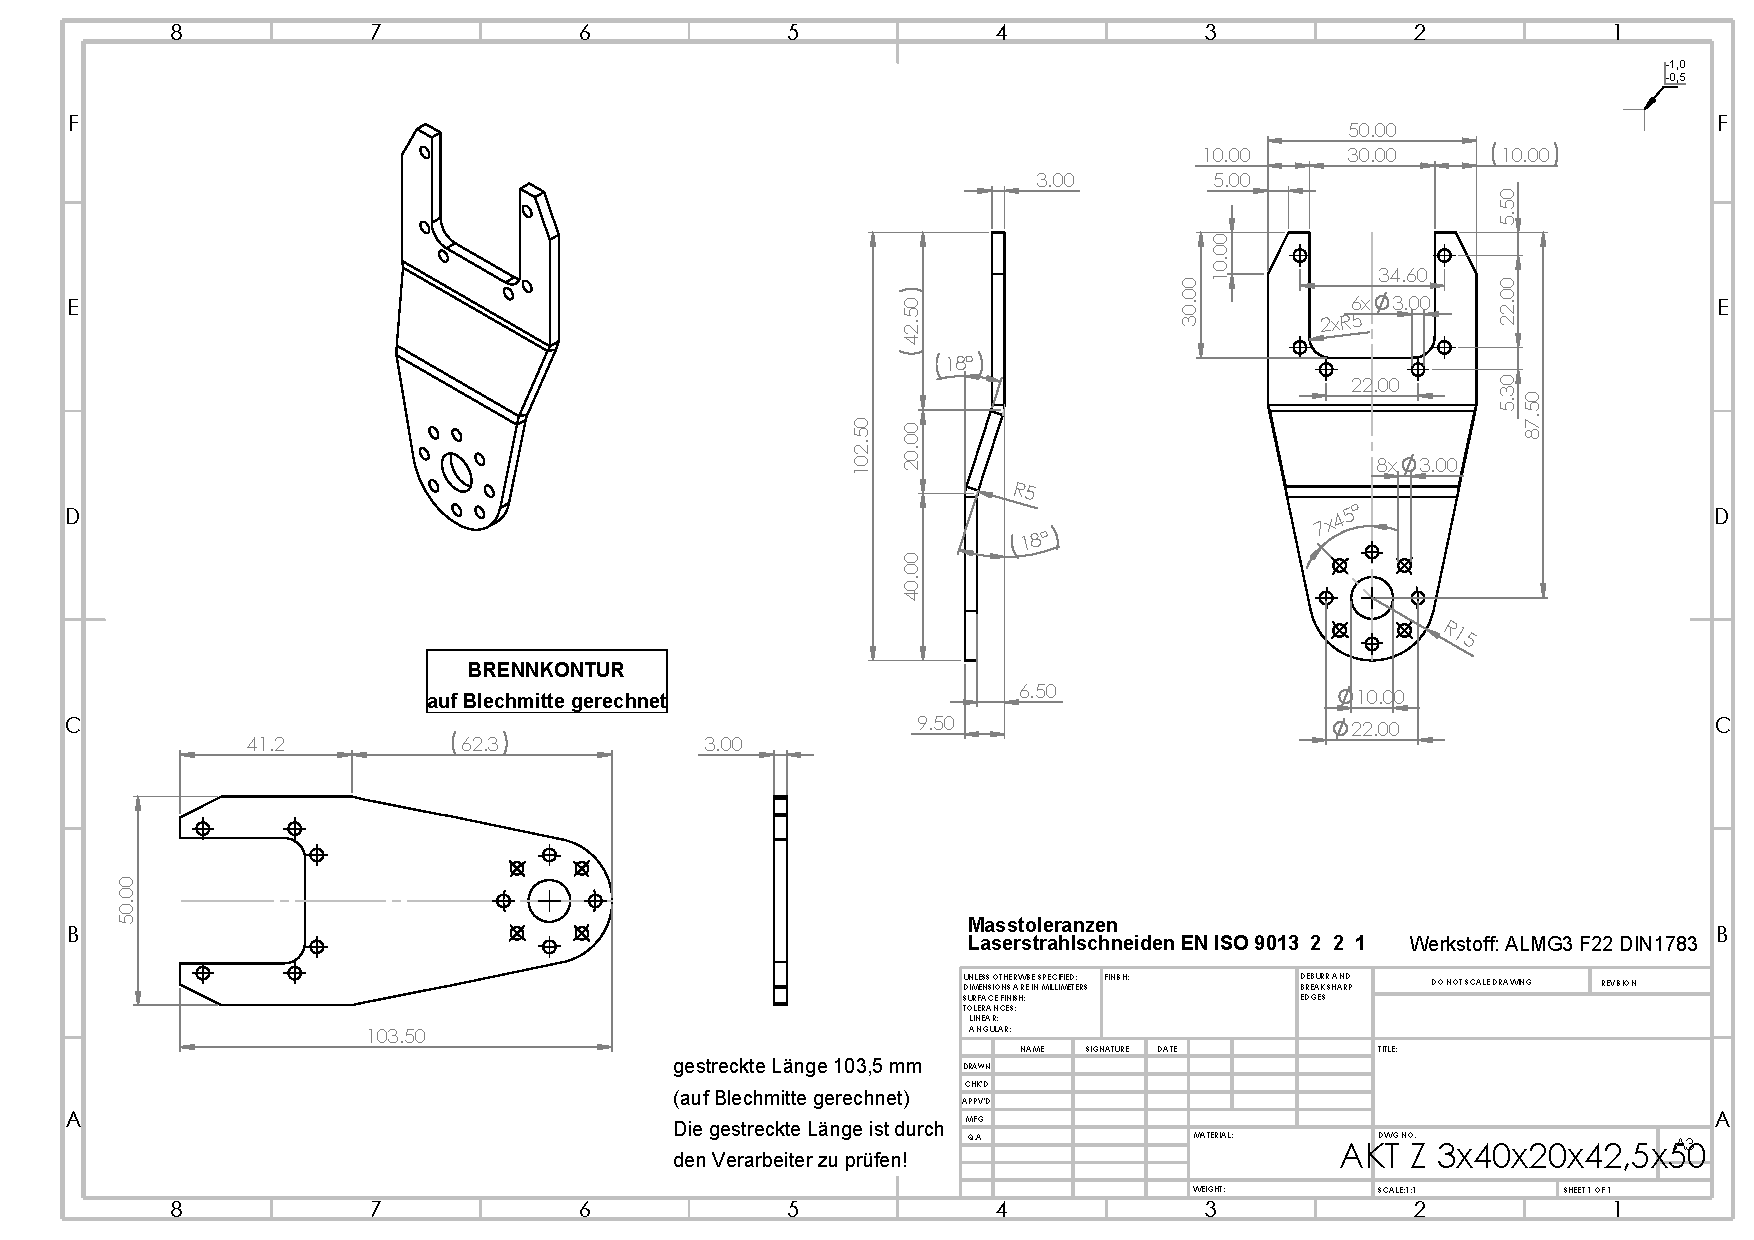
\includepdf[page=-]{../img/pdf/AKT Z 3x40x20x42_5x50.pdf}


\chapter{Motor Parameters}

\begin{table}[H]
	\centering
	\noindent\adjustbox{max width=\linewidth}{
		\begin{tabular}{|c|c|c|c|}
			\hline
			parameter & axis 0 & axis 1 & axis 2 \\
			\hline
			home offset & 2288 & 2060 & 3074 \\
			\hline
			min angle & 1580 & 2060 & 1650 \\
			\hline
			max angle & 3000 & 3200 & 3100 \\
			\hline
			max velocity & 20 & 20 & 20 \\
			\hline
			home & 2290 & 2060 & 3072 \\
			\hline
		\end{tabular}
	}
	\unterschrift{table of motor parameters}{}{}
	\label{tab:motor_param}
\end{table}



\end{document}